%% LyX 1.6.0 created this file.  For more info, see http://www.lyx.org/.
%% Do not edit unless you really know what you are doing.
\documentclass[english]{beamer}
\usepackage{mathptmx}
\usepackage[T1]{fontenc}
\usepackage[latin9]{inputenc}
\usepackage{amsmath}
\usepackage{amssymb}

\makeatletter
%%%%%%%%%%%%%%%%%%%%%%%%%%%%%% Textclass specific LaTeX commands.
 % this default might be overridden by plain title style
 \newcommand\makebeamertitle{\frame{\maketitle}}%
 \AtBeginDocument{
   \let\origtableofcontents=\tableofcontents
   \def\tableofcontents{\@ifnextchar[{\origtableofcontents}{\gobbletableofcontents}}
   \def\gobbletableofcontents#1{\origtableofcontents}
 }
 \makeatletter
 \long\def\lyxframe#1{\@lyxframe#1\@lyxframestop}%
 \def\@lyxframe{\@ifnextchar<{\@@lyxframe}{\@@lyxframe<*>}}%
 \def\@@lyxframe<#1>{\@ifnextchar[{\@@@lyxframe<#1>}{\@@@lyxframe<#1>[]}}
 \def\@@@lyxframe<#1>[{\@ifnextchar<{\@@@@@lyxframe<#1>[}{\@@@@lyxframe<#1>[<*>][}}
 \def\@@@@@lyxframe<#1>[#2]{\@ifnextchar[{\@@@@lyxframe<#1>[#2]}{\@@@@lyxframe<#1>[#2][]}}
 \long\def\@@@@lyxframe<#1>[#2][#3]#4\@lyxframestop#5\lyxframeend{%
   \frame<#1>[#2][#3]{\frametitle{#4}#5}}
 \makeatother
 \def\lyxframeend{} % In case there is a superfluous frame end

%%%%%%%%%%%%%%%%%%%%%%%%%%%%%% User specified LaTeX commands.
\usetheme{Warsaw}
% or ...

\setbeamercovered{transparent}
% or whatever (possibly just delete it)

\makeatother

\usepackage{babel}

\begin{document}

\title{Elliptic Curve Cryptography}


\author{G. Aleksandrowicz\inst{1} \and B. Hess\inst{2}\\Supervisor: Barukh Ziv}


\institute{\inst{1}Department of Computer Science, Technion \and \inst{2} Department of Computer Science, ETH Zurich}


%\date{Technion - Israel Institute of Technology\and \inst{2}Department
%of Theoretical Philosophy}


%\date{University of Else}


\date{Project in Computer Security, 2009}

\makebeamertitle

\lyxframeend{}

\lyxframe{Outline}

\tableofcontents{}

\lyxframeend{}

\section{Elliptic Curves}
\lyxframe{Definition}
\begin{itemize}
\item An Elliptic Curve is the set of solutions of an equation of the form
$y^{2}=x^{3}+ax+b$ over some field $\mathbb{F}$.
\item Usually denoted $E_{\mathbb{F}}$.
\item There is a small condition on $a,b$ ($4a^{3}+27b^{2}\ne0$)
\item If $\mbox{char}\mathbb{F}=2,3$ the equation is a little more complex...
\item We also consider a solution {}``at infinity'', $O$.
\end{itemize}
\lyxframeend{}

\lyxframe{The Group Operation - Illustration}
\begin{figure}[h]
\centering
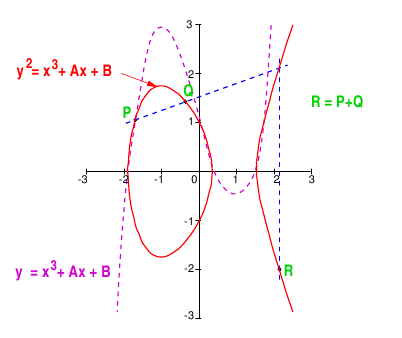
\includegraphics[scale=0.4]{ecaddition.png}
\caption{Addition of two points $P+Q$ in an EC}
\label{tradebefore}
\end{figure}
\lyxframeend{}

\lyxframe{Usage in Cryptography}
\begin{itemize}
\item Elliptic Curves provide a wide variety of groups, similar to $\mathbb{Z}_{n}^{*}$
but more complex.
\item Diffie-Hellman and El-Gamal can be reproduced in this setting.
\item The discrete logarithm problem is much harder - i.e. the index calculus
method is not applicable.
\item This results in much smaller key sizes (100-200 bits).
\item The problem: More costly to generate, more costly to operate.
\end{itemize}
\lyxframeend{}

\section{The Implementation}
\lyxframe{Our Goals}
\begin{itemize}
 \item Our main goal was to build an elliptic-curve cryptosystem from first principals.
 \item The only library used was an infinite integer precision library (GMP).
 \item The field arithmetic, elliptic curve operations and cryptosystem were all implemented by us.
 \item Greater control, flexability and understanding at a cost to efficiency.
 \item Optimizations can still be done by ``outsorcing`` parts of the code, after profiling.
 \item Another goal was experimenting with cutting-edge methods for generation of cryptographically secure elliptic curves.
 \item Again, everything was implemented ''from scratch`` (e.g. algorithms for modular polynomial root-finding, 2-adic field implementation and more).
\end{itemize}
\lyxframeend{}

\lyxframe{Representation of elliptic curve points}
\begin{itemize}
  \item Given an x-coordinate, there are only two possible corresponding y-coordinates.
  \item Hence coordinates are generally represented in the compressed form $\pm X$ with $X$ being the value of the x-coordinate and the sign
	specifying which of the two y-coordinates to choose.
  \item When performing calculations with points, it is more convenient to use Jacobian projective representation: $(X,Y,Z)$ corresponds to the point $(X/Z^2,Y/Z^3)$.
  \item This eliminates the need to perform the costly division operation during calculations (only in the final conversion).
\end{itemize}
\lyxframeend{}

\lyxframe{Encoding Text to an Elliptic Curve}
\begin{itemize}
 \item Our implementation encodes ASCII text to points on the EC.
 \begin{itemize}
  \item This is no restriction. Arbitrary files can be encoded to ASCII (e.g. with base64)
 \end{itemize}
 \item The encoding works the following way ($k$ is the maximum point size in bytes):
 \begin{itemize}
  \item $k-1$ characters are appended bytewise to the x-coordinate.
  \item 1 random byte is appended $\rightarrow$ padding.
  \item The corresponding y-coordinate is computed.
  \item If no y-coordinate exists, another random padding is selected.
 \end{itemize}
 \item Half of the x-coordinates correspond to a valid point.
 \item Padding serves two purposes:
 \begin{itemize}
  \item Finding a valid point
  \item Introducing non-determinism.
 \end{itemize}
\end{itemize}
\lyxframeend{}

\lyxframe{Binary field vs. prime field}
\begin{itemize}
  \item As mentioned, elliptic curves can be defined over any field.
  \item In practice, the fields used for cryptography are mainly $\mathbb{F}_{2^n}$ (a \emph{binary} field) and $\mathbb{F}_p$ (a \emph{prime} field).
  \item Both fields have different arithmetic and generation methods (e.g. for $\mathbb{F}_p$ we need a primality-testing algorithm).
  \item Generation of secure curves is a completely different problem for each of the cases.
  \item We have chosen to implement \emph{both} types of curves:
  \begin{itemize}
   \item Allows a comparision of the two methods.
   \item Enables us to explore the two theoretically interesting paths.
  \end{itemize}   
\end{itemize}
\lyxframeend{}

\lyxframe{Genration of secure curves}
\begin{itemize}
  \item The primary concern with a given elliptic curve concerns its order.
  \item It should be large enough, with few or none small factors, and satisfy some other properties to avoid specific attacks.
  \item Hence it is critical to be able to find the curve's order.
  \item In the binary field case this was done using the AGM method.
  \item In the prime field case a different approach was used: generate curves in a way such that the order is known in advance (the Complex multiplication method).
  \item There is also a general-purpose counting algorithm (Schoof's algorithm) but it is far more costly and complicated then our methods (although polynomial).
\end{itemize}

\lyxframeend{}

\lyxframe{The Complex Multiplication method}
\begin{itemize}
 \item Basic idea: given a prime $p$ and a negative integer $D$, it is possible to generate a curve from a root of a special polynomial (\emph{Hilbert class polynomial}) $H_D(x)$ over $\mathbb{F}_p$
 \item The resulting curve will have order $p+1-t$ or $p+1+t$ such that $t$ satisfies the equation $4p=t^2+|D|s^2$.
 \item The underlying theory is quite complex...
 \item In practice the main challenges are:
 \begin{itemize}
  \item Computing $H_D$ (difficult, requires high numerical precision; we can do with a list of pre-computed polynomials).
  \item Finding $p$ such that $4p=t^2+|D|s^2$ for random $t,s$ or find such $t,s$ with $p,D$ given (Cornacchia's algorithm).
  \item Computing a root of $H_D(x)$ modulo $p$ (requires algorithms for modular polynomial root-finding).
 \end{itemize}
\end{itemize}
\lyxframeend{}

\lyxframe{Point Counting with AGM (1)}
\begin{itemize}
\item The \emph{Arithmetic-Geometric Mean} is defined as the sequence:\end{itemize}
\begin{fact}%{}
$a_0=a$, $b_0=b$, $a_{n+1}=\frac{1}{2}(a_n+b_n)$, $b_{n+1}=\sqrt{a_nb_n}$\end{fact}%{}
\begin{itemize}
\item Gauss discovered: for $n\rightarrow\infty$, $a$ and $b$ will converge:\end{itemize}
\begin{fact}%{}
$AGM(a,b):=\lim\limits_{n \rightarrow \infty}{a_n}=\lim\limits_{n \rightarrow \infty}{b_n}$\end{fact}%{}
\begin{itemize}
\item Classical application of AGM: approximation of number $\pi$.
\end{itemize}

\lyxframeend{}

\lyxframe{Point Counting with AGM (2)}
\begin{itemize}
\item Mestre (2000) applied AGM for point counting in elliptic curves over $\mathbb{F}_{2^d}$, EC: $y^2+xy=x^3+c$
\item The EC order is determined by its \emph{trace} $t$: $|EC|=2^d+1-t$
\item $t$ is computed using AGM:
\end{itemize}
\begin{fact}$a=1$, $b=1+8c$, $t=\frac{a_0}{AGM(a,b)}=\frac{a_0}{a_d}$\end{fact}%{}
\begin{itemize}
\item Difficulty: $a$ and $b$ are so-called \emph{2-adic polynomials}
\item These are polynomials of degree $d$, with coefficients modulus $2^N$. $N$ is called the \emph{precision}.
\end{itemize}
\lyxframeend{}

\section{Results}

\lyxframe{ECC ElGamal Results}
\begin{figure}[h]
\centering
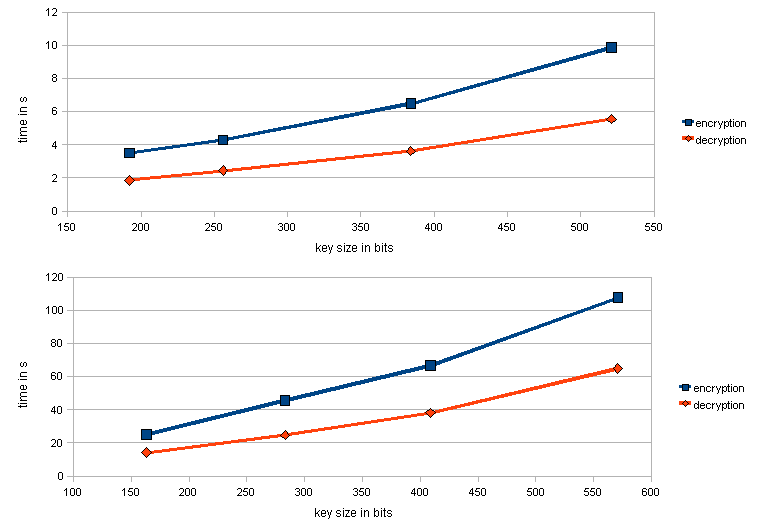
\includegraphics[scale=0.33]{dia2.png}
\caption{3.3KB file, top: prime curves, bottom: binary curves}
\label{agm1}
\end{figure}
\lyxframeend{}

\lyxframe{ECC ElGamal Evaluation}
\begin{itemize}
 \item Timings are not very competitive, there is much potential for optimizations.
 \item Both versions (binary and prime field) use field arithmetic, built from scratch.
 \begin{itemize}
  \item Using specialized libraries would improve the performance.
  \item Optimizations for reduction trinomials could be added in the binary case.
 \end{itemize}

\end{itemize}

\lyxframeend{}

\lyxframe{AGM implementation}
\begin{itemize}
\item Current programming libraries don't implement 2-adic arithmetic.
\item Our 2-adic implementation includes: addition/subtraction, multiplication, modular reduction, division, square root, inverse polynomial.
\item Polynomial multiplication is the major bottleneck. It can be highly optimized using FFT.
\item Comparison between AGM with ``naive'' multiplication and optimized variant from \emph{NTL} shows enormeous performance improvements:
\begin{itemize}
\item AGM on a 283 bit EC. Naive version: 30 minutes. Optimized version: 1.5 seconds.
\end{itemize}
\end{itemize}
\lyxframeend{}

\lyxframe{AGM Point Counting Evaluation}
\begin{figure}[h]
\centering
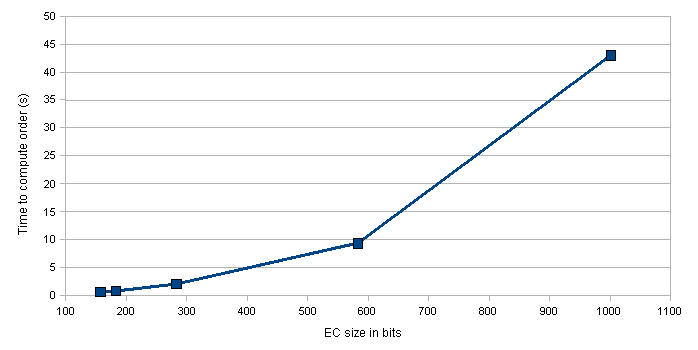
\includegraphics[scale=0.35]{dia1.png}
\caption{AGM times with variable EC sizes, 1.8GHz Core Duo}
\label{agm1}
\end{figure}
\lyxframeend{}

\lyxframe{Challenge}
\begin{itemize}
  \item We were given messages encrypted using a prime field for a given $p$ (the 13-th Mersenna prime)
  \item Some information on the curves used was given (Generated using the CM method, with $D>-400$ and good security parameters)
  \item A complete search yielded exactly one suitable curve (i.e. satisfying the security constraints for $p$).
  \item This made full use of the ability to calculate the group order using the CM method and finding the decomposition $4p=t^2+|D|s^2$.
  \item Inside the decrypted messages was yet another encryption, this time over a binary field.
  \item Our implementation decrypted the inner message as well.
\end{itemize}

\lyxframeend{}

\section{Further Work}
\lyxframe{CM method - Further work}
  \begin{itemize}
    \item Validating the correct of the two possible orders was done in a brute-force (but efficient) way - this can be improved.
    \item We can investigate ways to efficiently generate the Hilbert class polynomials.
  \end{itemize}
\lyxframeend{}

\lyxframe{AGM - Further Work}
\begin{itemize}
\item Not all random curves are secure. Curve order should exceed a certain value.
\begin{itemize}
\item Use a ``early abort'' strategy to quickly skip insecure curves.
\end{itemize}
\item Even faster libraries for polyomial multiplication exist today
\begin{itemize}
 \item Use ``FLINT'' instead of NTL.
\end{itemize}
\item Other point counting methods exist, with lower asymptoic complexity.
\begin{itemize}
 \item AGM has $O(n^{3+\epsilon})$ complexity.
 \item Newer method has $O(n^{2+\epsilon})$ complexity.
 \item Practical comparison would be interesting.
\end{itemize}
\item Comparison with binary field CM.
\end{itemize}
\lyxframeend{}


\appendix

\section*{Appendix}


\lyxframeend{}\subsection*{For Further Reading}


\lyxframeend{}\lyxframe{[allowframebreaks]For Further Reading}

\beamertemplatebookbibitems
\begin{thebibliography}{1}
\bibitem{HMV}D. Hankerson, A. Menezes, S. Vanstone. Guide to Elliptic
Curve Cryptography. Springer, 2004.
\bibitem{HMV}H. Baier, J. Buchmann. Generation Methods of Elliptic Curves. 2002.	\beamertemplatearticlebibitems

\end{thebibliography}

\lyxframeend{}
\end{document}
